% Template for ICIP-2015 paper; to be used with:
%          spconf.sty  - ICASSP/ICIP LaTeX style file, and
%          IEEEbib.bst - IEEE bibliography style file. cambio para probar adsfasfasfasfsf
% --------------------------------------------------------------------------
\documentclass[spanish,twocolumn]{article}
\usepackage{spconf,amsmath,graphicx}
\usepackage{mathptmx}
\usepackage{mathtools}
\usepackage{amsmath}
\usepackage{mathrsfs}
\usepackage{amssymb}
\usepackage{amsfonts}
\usepackage[utf8]{inputenc}
\usepackage{babel}
\usepackage{color}
\usepackage[Algoritmo]{algorithm}
\usepackage{algpseudocode}
\usepackage{multicol}
\usepackage{caption,setspace}
\usepackage{subfig}
\usepackage{graphicx}

\algrenewcommand\algorithmicif{\textbf{si}}
\algrenewcommand\algorithmicend{\textbf{fin}}
\algrenewcommand\algorithmicfor{\textbf{para}}
\algrenewcommand\algorithmicdo{\textbf{hacer}}
\algrenewcommand\algorithmicwhile{\textbf{mientras}}
\algrenewcommand{\algorithmicrequire}{\textbf{Entrada:}}
\algrenewcommand{\algorithmicensure}{\textbf{Salida:}}
\selectlanguage{spanish}
% Example definitions.
% --------------------
\def\x{{\mathbf x}}
\def\L{{\cal L}}

% Title.
% ------
\title{OPTIMIZACIÓN MULTIOBJETIVO BASADA EN LA SINTONIZACIÓN DE LOS PARÁMETROS DE CLAHE PARA OBTENER DISTINTOS NIVELES DE CONTRASTE EN IMÁGENES MÉDICAS}
%\title{OPTIMIZACIÓN MULTIOBJETIVO PARA LA MEJORA DEL CONTRASTE BASADA EN CLAHE.}
%
% Single address.
% ---------------
\name{Luis G. Moré, Marcos A. Brizuela, Horacio Legal Ayala, Diego Pinto-Roa, José Luis Vázquez Noguera}
\address{Facultad Politécnica - Universidad Nacional de Asunción}
%
% For example:
% ------------
%\address{School\\
%	Department\\
%	Address}
%
% Two addresses (uncomment and modify for two-address case).
% ----------------------------------------------------------
%\twoauthors
%  {A. Author-one, B. Author-two\sthanks{Thanks to XYZ agency for funding.}}
%	{School A-B\\
%	Department A-B\\
%	Address A-B}
%  {C. Author-three, D. Author-four\sthanks{The fourth author performed the work
%	while at ...}}
%	{School C-D\\
%	Department C-D\\
%	Address C-D}
%
\begin{document}
%\ninept
%
\maketitle
%
\begin{abstract}
En determinadas imágenes médicas, es posible lograr una mejora de contraste a distintos niveles, de manera a resaltar distintas estructuras presentes en las mismas. Ésto podría resultar útil a los especialistas médicos para realizar diagnósticos más específicos, como por ejemplo en radiografías del tórax y mamografías, en donde se pueden resaltar distintos detalles de la imagen de acuerdo al contraste obtenido. Se propone la sintonización de parámetros de Contrast Limited Adaptive Histogram Equalization(CLAHE), utilizando una metaheurística multiobjetiva. Los objetivos propuestos son maximizar la cantidad de información disponible (por medio de la Entropía) y minimizar la distorsión en las imágenes resultantes (Índice de Similitud Estructural) de manera simultánea. Los resultados muestran un conjunto de soluciones o Conjunto Pareto, que representa a la imagen con distintos niveles de contraste y distintos niveles de compromiso entre Entropía e Índice de Similitud Estructural, lo que muestra que éstos objetivos son contradictorios. 
%La mejora del contraste en imágenes médicas presenta desafíos importantes, debido a que se necesita realzar los detalles y también preservarlos, de forma a que la mejora sea de ayuda para análisis posteriores. Se propone un enfoque de mejora multiobjetivo basada en CLAHE, utilizando SMPSO como metaheurística, además de la Entropía y el SSIM como objetivos, de manera a maximizar el contraste y minimizar la distorsión de los resultados. Se obtienen distintos niveles de contraste en imágenes de radiografía del tórax, y así se resaltan distintos detalles de éstas. Los resultados obtenidos se analizan con ayuda de un especialista de manera a determinar la utilidad del enfoque, además se verifica que los objetivos son contradictorios.
\end{abstract}
%
\begin{keywords}
SMPSO, CLAHE, Entropía, SSIM, Mejora del Contraste, Optimización.
\end{keywords}
%
\section{Introducción}
\label{sec:intro}

Es de gran importancia realizar la Mejora del Contraste de imágenes de carácter médico, debido a que de esta manera es posible acentuar y mantener las características presentes en ellas. Las radiografías presentan características particulares de contraste, como en el caso de radiografías del tórax y mamografías, donde pueden existir diferencias de constraste notorias debido a las características de atenuación de los Rayos X \cite{chang1998image}.%; además de que las técnicas de mejora de contraste pueden ayudar a reducir la dosis de radiación aplicada para obtener la imagen \cite{zhang2009mammograms}.

Existen diversas propuestas de Mejora del Contraste basadas en transformaciones del Histograma \cite{1658094}. Los enfoques de mejora local demuestran ser sumamente útiles al momento de realzar detalles en imágenes médicas, y existen diversas propuestas que se centran en mejorar el contraste en radiografías \cite{1625082,4712472,5360176}. En nuestra propuesta se utilizará una metaheurística de optimización de objetivos, de manera a sintonizar los parámetros de entrada del algoritmo de mejora del contraste descripto en la sección \ref{sec:clahe}, de manera a obtener un grupo de imágenes contrastadas, las cuales serán evaluadas en cuanto a la ganancia de información proveída y distorsión introducida por la ecualización (sección \ref{sec:metricas}). Se generan imágenes con distintas relaciones entre contraste y distorsión, de manera a resaltar características distintas de las imágenes de prueba, lo cual resulta de utilidad para el análisis realizado por el especialista.
 En la literatura existen propuestas de mejora basadas en metaheurísticas, como se ve en \cite{Hashemi20101816}, en el que se utilizan Algoritmos Genéticos, en \cite{morebrizuela2014} se utiliza un enfoque muy similar a la propuesta presentada, aunque se enfoca a un solo objetivo, y solamente se obtiene un resultado por cada imagen original, o en \cite{Shanmugavadivu2014243}, en donde también se utiliza una metaheurística multiobjetiva; la principal diferencia radica en que nuestra propuesta se aplica de manera más efectiva en imágenes médicas, debido a que CLAHE muestra resultados satisfactorios en éste tipo de imágenes \cite{reza2004,5360176}, además de mostrar los mejores resultados de forma automática. 

%Se pueden encontrar distintas técnicas de mejora del contraste, las cuales son en su mayoría transformaciones basadas en la Ecualización del Histograma\cite{russ2010image,841534}. En su forma clásica, la Ecualización del Histograma se puede considerar como una transformación de enfoque global, debido a que la información de todos los pixeles que conforman la imagen se tienen en cuenta en el proceso de ecualización \cite{1419470}. Sin embargo, este enfoque no es aplicable para imágenes con características de contraste heterogéneas \cite{841534}. Realizar la mejora del contraste teniendo en cuenta sectores de la imagen es más importante cuando se tienen detalles muy finos, por tanto se tuvo en cuenta un algoritmo de mejora local, el cual posee parámetros que necesitan de ajuste de manera a aumentar la utilidad de los resultados. Además es necesario considerar métricas que permitan evaluar los resultados en términos de realce y de calidad de detalles, por lo que es necesario considerar la mejora del contraste como un problema de optimización.


El resto del trabajo se organiza de la siguiente manera: En la sección \ref{sec:clahe} se describe brevemente el algoritmo de mejora de contraste adoptado; en la sección \ref{sec:metricas} se muestran las métricas de evaluación de resultados utilizadas; en la sección \ref{sec:formulacion} se plantea de manera formal el problema que se intenta resolver; en la sección \ref{sec:propuesta} se muestra cómo se aplica la optimización al algoritmo de mejora del contraste; luego en la sección \ref{sec:resultadosdiscusion} se discuten los resultados, y finalmente en la sección \ref{sec:conclusion} se detallan las conclusiones correspondientes. 


%\section{PSO-CLAHE MULTIOBJETIVO}
%\label{sec:psoclahe}

%En esta sección se describe el enfoque empleado para resolver el problema que se plantea. En \cite{morebrizuela2014} se muestra una implementación orientada a la optimización monoobjetivo, por ende se obtiene un solo resultado para cada ejecución de la implementación. Aquí se muestra cómo se extendió el trabajo para obtener varios resultados con distintos niveles de contraste. Las imágenes se evalúan de acuerdo a las métricas de evaluación descritas en las secciones subsiguientes, las cuales conforman funciones objetivo para la metaheurística de optimización, como también se describe en la sección \ref{sec:formulacion}.

\section{Contrast Limited Adaptive Histogram Equalization}
\label{sec:clahe}
Este enfoque de mejora de contraste presentado en \cite{Zuiderveld:1994:CLA:180895.180940} es una extensión del algoritmo original Adaptive Histogram Equalization (AHE) \cite{pizer1987adaptive}; en ambos métodos se implementa una Ecualización del Histogama basada en {\it Regiones Contextuales} cuyas dimensiones están delimitadas por $(\mathcal{R}_x, \mathcal{R}_y)$, para realizar la ecualización en varios sectores de la imagen. Las inconsistencias entre fronteras de la imagen se corrigen aplicando interpolación bilineal. AHE presenta problemas de amplificación del ruido, entonces en CLAHE se implementa una limitación en el contraste a través de la limitación de la cantidad de pixeles que pueden alcanzar cierto nivel de gris dentro del histograma local; aquí se define el coeficiente {\it Clip Limit} $\mathcal{C}$ como un factor que está fuertemente relacionado con los contenidos del histograma. %Si definimos un coeficiente $\mathcal{C}$ relativamente bajo, entonces los histogramas de las regiones contextuales no muestran picos, por lo que se obtiene una mejora del contraste relativamente suave. Si definimos un $\mathcal{C}$ alto, obtenemos un comportamiento de $CLAHE$ que resulta ser equivalente al algoritmo $AHE$. En el contexto del trabajo propuesto, la selección de parámetros de CLAHE es fundamental para lograr resaltar los detalles en radiografías, y evitar una amplificación en el ruido indeseable \cite{pisano1998}.

\section{métricas de evaluación}
\label{sec:metricas}

Para cada resultado obtenido por CLAHE, es necesario utilizar métricas que permitan determinar cuantitativamente la calidad de las imágenes resultantes; es por esto que adoptamos dos métricas que consideramos importantes para las comparaciones entre resultados; éstas son la Entropía como medida de mejora del contraste, y el Índice de Similitud Estructural como medida de distorsión de la imagen.

\subsection{Entropía}
\label{ssec:entropia}

La {\it Entropía de la Información} es una medida de la aleatoriedad presente en la imagen \cite{tsai2008information}. Se puede definir la Entropía de la imagen como: % Al medir la Entropía de una imagen, se puede ver el desorden en la distribución de niveles de gris del histograma. Si definimos el histograma de una imagen en niveles de gris, como se muestra abajo: 

%\begin{equation}\label{eq:histograma}
%    \mathcal{H}=\{h_i \in [0...N]\mid i=0,1,...,L-1\}
%\end{equation}

%donde $h_i$ es el recuento de apariciones del $i-esimo$ nivel de gris componente de la imagen; $N$ es el número total de pixeles que componen la imagen (aquí, $N=\sum_{i=0}^{L-1}h_i$); $L$ representa al nivel de gris más alto que puede utilizar para representar la imagen;  además, si la distribución normal de niveles de gris en el histograma se define como $\mathcal{P}_i=\frac{h_i}{N}$ entonces se puede definir la Entropía de la imagen como:

%\begin{equation}\label{eq:distribucionormal}
%\mathcal{P}_i=\frac{h_i}{N}
%\end{equation}

%entonces se puede definir la Entropía de la imagen como:

\begin{equation}\label{eq:entropia}
\mathscr{H}=-\sum_{i=0}^{L-1}\mathcal{P}_i log_2(\mathcal{P}_i) [bits] \quad \mathscr{H} \in {0,..,log_2(L)} 
\end{equation}

Donde $\mathcal{P}_i$ es la probabilidad de ocurrencias del nivel de gris $i$ en el histograma y $L$ es el máximo nivel de gris que se puede utilizar para representar la imagen. Esta métrica es interesante debido a que está fuertemente asociada al brillo medio de la imagen \cite{108593}; este coeficiente nos ayuda a ver cuánto aumenta el contraste como consecuencia de la transformación de la imagen.

\subsection{Índice de similitud estructural}
\label{ssec:ssim}

El {Índice de Similitud Estructural (SSIM)} \cite{wang2004image} es un coeficiente que mide el grado de distorsión producida en una imagen resultante $T$ a consecuencia de aplicar una Mejora del Contraste a una imagen original $I$. SSIM se calcula por bloques, por lo que si definimos dos ventanas $I_x$ e $T_y$ para las imágenes original y resultante, respectivamente, se define el SSIM como se muestra abajo:



\begin{equation}\label{eq:ssim}
\resizebox{.9\hsize}{!}
{
$SSIM(I,T)=\frac{(2\mu_{I_x}\mu_{T_y}+C_1)(2\sigma_{I_xT_y}+C_2)}{(\mu_{I_x}^2+\mu_{T_y}^2+C_1)(\sigma_{I_x}^2+\sigma_{T_y}^2+C_2)} \quad SSIM \in [0,1]$
}
\end{equation}

Donde $\mu_{I_x}$ es el promedio de intensidades de $I_x$; $\mu_{T_y}$ es el promedio de intensidades de $T_y$; $\sigma_{I_x}^2$ y $\sigma_{T_y}^2$ son las varianzas de intensidades de $I_x$ e $T_y$, respectivamente; $\sigma_{I_x T_y}$ es la covarianza entre $I_x$ e $T_y$; $C_1=(K_1L^2)$, $L$ es el rango dinámico de intensidades de los pixeles (256 para una imagen en escala de grises de 8 bits) y $K_1 \ll 1$ es una constante pequeña; $C_2=(K_2 L)^2$, y $K_2 \ll 1$; tanto $C_1$ y $C_2$ son constantes que se usan para estabilizar la division en caso de que el denominador tienda a cero.

\begin{algorithm}[H]
    \scriptsize
    \begin{algorithmic}[1]
        \Require imagen de entrada $I$, número de partículas $\Omega$, número de iteraciones $t_{max}$
        \State Inicializar los parámetros $\omega$, $C_1$, $C_2$, $t=0$, $lower\_limit_1$, $lower\_limit_2$, $lower\_limit_3$, $upper\_limit_1$, $upper\_limit_2$, $upper\_limit_3$, $\mathscr{X}$
        %\For{cada $i$-ésima partícula del enjambre}
        %    \State Inicializar la posición $x_i$ aleatoriamente
        %    \State Inicializar la velocidad $v_i$ a 0
        %    \State ${imagenMejorada}$ = CLAHE(${x_i}$, ${imagenOriginal}$)
        %    \State ${f_i}$ = evaluarAptitud(${imagenOriginal}$, ${imagenMejorada}$)
        %    \State Establecer el mejor individual inicial $p_i$ por el valor inicial $x_i$
        %    \If{$f_i < f_{p_g}$}
        %        \State reemplazar $p_g$ por el valor de $x_i$
        %    \EndIf
        %\EndFor
        \While{$t$ $<$ $t_{max}$}
            \For{cada $i$-ésima partícula del enjambre}
                \State Calcular la nueva velocidad de la partícula $\overrightarrow{v_i}^t$ utilizando la ecuación \eqref{eq:psobasico2}, sujeto a las restricciones impuestas por \eqref{eq:restricciondelta}

%                \begin{equation*}\label{eq:psobasico2}
%                    \overrightarrow{v_i}(t) = \omega \cdot \overrightarrow{v_i} \cdot (t-1) + C_1 \cdot r_1 \cdot (\overrightarrow{x_{p_i}}-\overrightarrow{x_i}) + C_2 \cdot r_2
%                \end{equation*}



                \State Calcular la nueva posición de la partícula $\overrightarrow{x_i}^t$ con la expresión de posición \eqref{eq:psobasico}
                %\begin{equation*}\label{eq:psobasico}
                %    \overrightarrow{x_i}(t) = \overrightarrow{x_i}(t-1) + \overrightarrow{v_i}(t)
                %\end{equation*}

                \State ${T}$ = CLAHE(${\overrightarrow{x_i}^t}$, ${I}$)
                \State ${f^t_i}$ = $f(I, \overrightarrow{x_i}^t)$%evaluarAptitud(${I}$, ${T}$)
                \If{$f^t_i < f_{\overrightarrow{x}_{p_i}}$}
                    \State reemplazar $\overrightarrow{x}_{p_i}$ por el nuevo valor de $\overrightarrow{x_i}^t$
                \EndIf
                \If{$ \overrightarrow{x_i} \succ \overrightarrow{x_{g_i}}$  }
                    \State actualizar $\mathscr{X}$
                \EndIf
                \State $t$ = $t$ + 1
            \EndFor
        \EndWhile
    \Ensure $\mathscr{X}$
    \end{algorithmic}
    \caption{Algoritmo $PSO-CLAHE$ Multiobjetivo.}
    \label{alg:pso_clahe}
\end{algorithm}

\section{Formulación del Problema Planteado}
\label{sec:formulacion}

Dadas la imagen de entrada $I$, y un vector $\overrightarrow{x}=(\mathcal{R}_x, \mathcal{R}_y, \mathcal{C})$, donde $\mathcal{R}_x$ y $\mathcal{R}_y$ conforman la región contextual y $\mathscr{C}$ es el $Clip Limit$, se desea calcular el conjunto de soluciones $\mathscr{X}$ que maximice de manera simultánea los objetivos $f_1$ y $f_2$, como se muestra abajo:

\begin{equation}\label{eq:fitness}
    f(I, \overrightarrow{x}) = \{ f_1(I, \overrightarrow{x}), f_2(I, \overrightarrow{x}) \} \qquad f_1,f_2 \in [0,1]
\end{equation}

donde:
\begin{itemize}
%\item $\overrightarrow{x}=(\mathcal{R}_x, \mathcal{R}_y, \mathcal{C})$, donde $\mathcal{R}_x$ y $\mathcal{R}_y$ conforman la región contextual y $\mathscr{C}$ es el Clip Limit.
\item $f_{1}(I, \overrightarrow{x})=\frac{\mathscr{H}(T)}{log_{2}L}$ es la Entropía normalizada de la imagen $T$.%, y $L$ la cantidad de grises disponibles.
\item $f_{2}(I, \overrightarrow{x})=SSIM(I,T)$ es el Índice de Similitud Estructural entre $I$ y $T$.

Siendo $T$ la imagen mejorada por $CLAHE(\overrightarrow{x},I)$ con los parámetros dados por $\overrightarrow{x}$ aplicados a $I$.

\end{itemize}

sujeto a:

\begin{itemize}
\item $\mathcal{R}_x \in [2,..,M]$ en los números $\mathbb{N}$.
\item $\mathcal{R}_y \in [2,..,N]$ en los números $\mathbb{N}$.
\item $\mathscr{C} \in (0,1]$ en los números $\mathbb{R}$.
\end{itemize}

Ésto significa que los valores de $\mathcal{R}$ solamente pueden tomar valores enteros positivos entre $(2,2)$ y $(M,N)$ y que $\mathscr{C}$ puede tomar un valor mayor a cero y menor o igual a 1.


\section{propuesta}
\label{sec:propuesta}
Se utiliza el algoritmo $SMPSO$ \cite{4938830}, donde las soluciones potenciales $\overrightarrow{x}=(\mathcal{R}_x, \mathcal{R}_y, \mathcal{C})$ se denominan {\it partículas} y el conjunto de partículas $\Omega$ se denomina {\it enjambre}. Cada partícula $\overrightarrow{x_i}$ se actualiza en cada generación $t$ de acuerdo a la siguiente ecuación:

\begin{equation}\label{eq:psobasico}
\overrightarrow{x_i}^t = \overrightarrow{x_i}^{(t-1)} + \overrightarrow{v_i}^t
\end{equation}

donde el factor $\overrightarrow{v_i}$ se conoce como la velocidad y está dado por:

\begin{equation}\label{eq:psobasico2}
\overrightarrow{v_i}^t = \omega \cdot \overrightarrow{v_i}^{(t-1)} + C_1 \cdot r_1 \cdot (\overrightarrow{x_{p_i}}-\overrightarrow{x_i}) + C_2 \cdot r_2 \cdot (\overrightarrow{x_{g_i}}-\overrightarrow{x_i})
\end{equation}

Aquí, $\overrightarrow{x_{p_i}}$ es la mejor solución que encontró $\overrightarrow{x_i}$, $\overrightarrow{x_{g_i}}$ es la mejor partícula (también conocida como {{\it líder}) que se encuentra en todo el enjambre, $\omega$ es el peso de la inercia de la partícula, $r_1$ y $r_2$ son dos números aleatorios, y $C_1$ y $C_2$ son son parámetros que controlan el efecto de las partículas locales  y globales. Si una partícula es mejor que otra, se dice que la $domina$, y la dominancia está definida de la siguiente manera: $\overrightarrow{x_{g_i}} \succ \overrightarrow{x_i}$ si y sólo si

\begin{equation}\label{eq:dominanciapareto}
         \begin{cases}  f_i(I,\overrightarrow{x_{g}})  \geq f_i(I,\overrightarrow{x}) \forall i \in \{1,2\} \\
                        f_i(I,\overrightarrow{x_{g}}) > f_i(I,\overrightarrow{x}) \exists i \in \{1,2\} \\
         \end{cases}
\end{equation}

El {\it Conjunto Pareto} es el grupo de soluciones $\mathscr{X}$, y la imagen en el espacio objetivo es el {\it Frente Pareto}.

En adición, en $SMPSO$ se realiza una restricción en $\overrightarrow{v}$, para cada componente $j$ de $\overrightarrow{x}$, de acuerdo a la siguiente ecuación: 
                
\begin{equation}\label{eq:restricciondelta}
    v_{i,j}^t = \begin{cases}  delta_j &\mbox{if } v_{i,j}^t > delta_j \\
                                -delta_j & \mbox{if } -delta_j \\
                                v_{i,j}^t & otherwise \end{cases}
\end{equation}

donde: 
\begin{equation} \label{eq:restricciondelta2}
delta_j= \frac{upper\_limit_j - lower\_limit_j}{2}
\end{equation}

El \textbf{Algoritmo \ref{alg:pso_clahe}} muestra cómo se implementa la propuesta. Las imágenes resultantes se evalúan de acuerdo a las métricas \eqref{eq:entropia} y \eqref{eq:ssim}, y los mejores resultados que se obtienen en base a éstas métricas conforman un conjunto pareto de soluciones. El conjunto representa una serie de imágenes con distintos niveles de contraste, de manera a resaltar características particulares de la misma.

La interacción entre CLAHE y las partículas de SMPSO se muestran en la \textbf {Fig. 1}. CLAHE recibe como parámetros de entrada los valores almacenados por una partícula $(\mathcal{R}_x,\mathcal{R}_y, \mathscr{C})$ y la imagen original $I$, y a la imagen procesada se le calculan las métricas $\mathscr{H}$ y $SSIM$ de manera a obtener las funciones objetivo. Las soluciones no dominadas se almacenan en el conjunto pareto. Éste proceso se repite hasta alcanzar un criterio de parada definido.

\begin{minipage}[b]{1.0\linewidth}
  \vspace{0.5cm}
  \centering
  \centerline{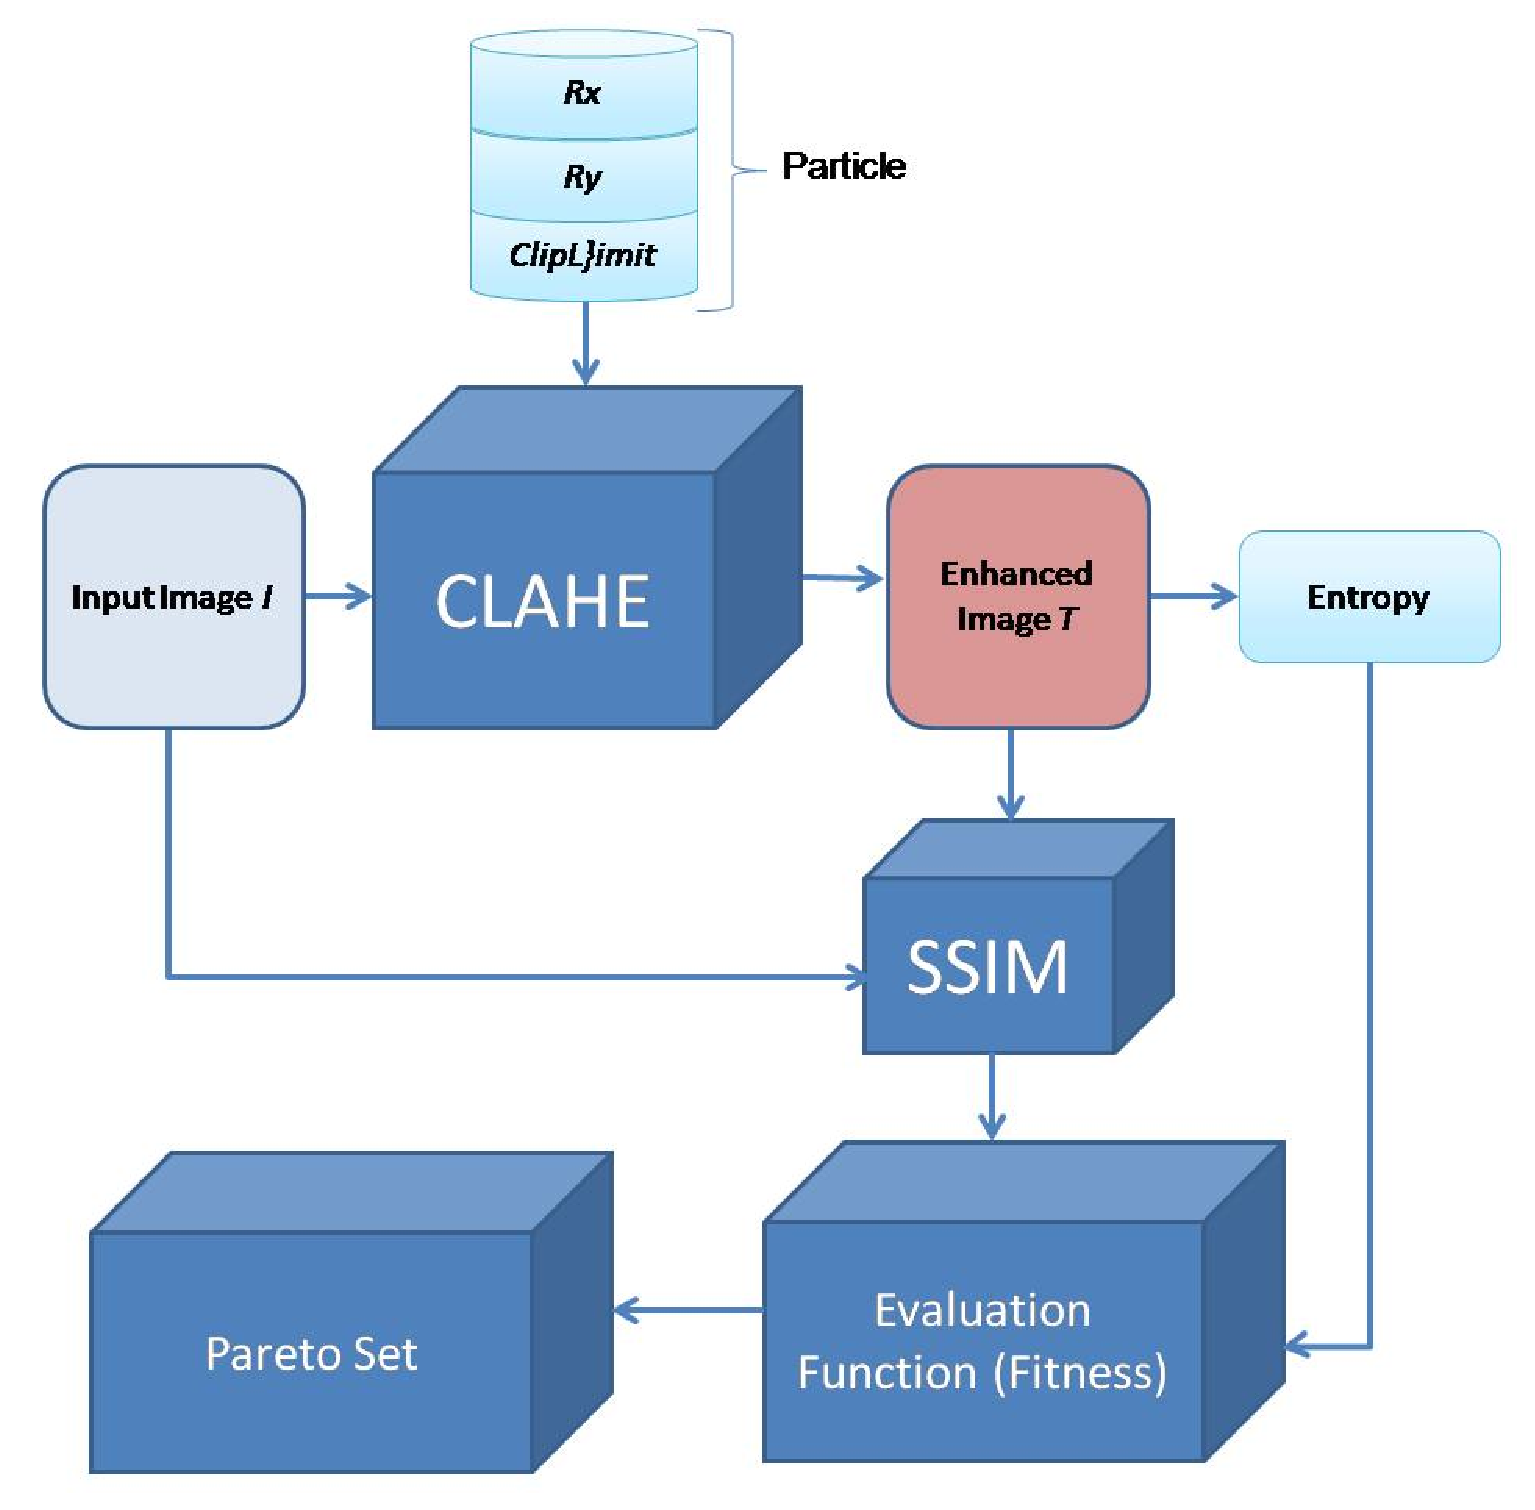
\includegraphics[height=6.5cm]{Figures/particula_clahe2}}
  \vspace{0.5cm}
  \label{fig:particula_clahe}
  \captionof{figure}{Interacción entre CLAHE y SMPSO.}
\end{minipage}

\section{resultados y discusión}
\label{sec:resultadosdiscusion}


Para la ejecución se utilizó como hardware una laptop con procesador Intel Core i3 de doble núcleo, con 2,5 GB de memoria RAM, y sistema operativo Windows 7 de 32 bits. La metaheurística $SMPSO$ está disponible en \cite{5586354}; mientras que la implementación de $CLAHE$ y de las métricas $\mathscr{H}$ y $SSIM$ se encuentran en \cite{opencv_library}. Se realizaron pruebas contra {\color{red} 16} imágenes de radiografía del tórax y mamografías, de manera a comprobar la efectividad de la propuesta; las mismas se descargaron del sitio http://openi.nlm.nih.gov/.  Se escogieron parámetros iniciales como se muestra en la \textbf{Table \ref{table:parametrospso}}:

\begin{table}[h]
\begin{center}
 \begin{tabular}{||c c | c c||} 
 \hline
 Parametro & Valor & Parametro & Valor \\ [0.5ex] 
 \hline\hline
 $lower\_limit_{\mathscr{R}_x}$ & $2$ & $upper\_limit_{\mathscr{R}_x}$ & $M/2$ \\ 
 \hline
 $lower\_limit_{\mathscr{R}_y}$ & $2$ & $upper\_limit_{\mathscr{R}_y}$ & $N/2$ \\  
 \hline
 $lower\_limit_{\mathscr{R}_{\mathscr{C}}}$ & $0$ & $upper\_limit_{\mathscr{R}_{\mathscr{C}}}$ & $0,5$ \\
\hline
$\Omega$ & $100$ & $t$ & $100$ \\ 
\hline
$C_1$ Min & $1,5$ & $C_1$ max & $2,5$ \\ 
\hline
$C_2$ Min & $1,5$ & $C_2$ max & $2,5$ \\ 
\hline
$r_1$ Min & $0,0$ & $r_1$ max & $1,0$ \\ 
\hline
$r_2$ Min & $0,0$ & $r_2$ max & $1,0$ \\ [1ex]
\hline
\end{tabular}
\end{center}
\caption[Parámetros de entrada para $SMPSO$]{Parámetros de entrada para $SMPSO$}
\label{table:parametrospso}
\end{table}
 

 Se realizaron 30 ejecuciones por cada imagen de prueba. Se obtuvieron aproximadamente 300 imágenes soluciones pareto por cada una de ellas, lo que representa un amplio grupo de imágenes a diferentes niveles de contraste y distorsión, lo que facilitaría el análisis de las mismas. En \textbf {Fig. 2}  y \textbf {Fig. 3}  se muestran 2 de las soluciones que se que se encuentran en el conjunto pareto, de manera a ejemplificar visualmente cuál es la variación de contraste que se obtiene, además de la imagen original como referencia. En \textbf {Fig. 4} se puede notar una relación inversa entre los objetivos, es decir al aumentar el coeficiente de entropía disminuye el SSIM; lo cual indica que estas dos métricas se complementan para mantener el compromiso entre aumento de contraste y minimización de la distorsión. Del Frente Pareto se pueden extraer imágenes que permiten visualizar determinados detalles de acuerdo a cómo varía el contraste logrado.  Se puede notar también que en las radiografías del tórax se aprecian mejor los tejidos blandos al alcanzar determinado contraste (véase \textbf {Fig.} 2b ) y a su vez las estructuras óseas se vuelven más visibles al alcanzar determinado contraste (véase \textbf {Fig.} 2c). Se logra un efecto similar en las imágenes de mamografía (véase \textbf {Fig.} 3b), en donde las potenciales lesiones se hacen más visibles, aunque se mantienen los detalles finos de las imágenes de manera satisfactoria. En nuestra propuesta se obtiene una cantidad importante de imágenes resultantes con distintas relaciones entre contraste y distorsión de manera automática, lo cual representa una ventaja porque se evita configurar los parámetros de mejora de forma arbitraria, como ocurre en \cite{1419470}.

\section{conclusiones}
\label{sec:conclusion}
Se presenta un algoritmo metaheurístico que maximiza de manera simultánea el contraste por medio de la Entropía y el Índice de Similitud Estructural, con ésto último se logra minimizar la distorsión de la imagen, en el contexto de las imágenes médicas, específicamente en imágenes de radiografías del tórax y mamografías. Los resultados experimentales muestran un conjunto de soluciones a diferentes niveles de contraste que permiten ver diferentes estructuras. Ésto permitiría a los médicos tener diferentes opciones de visualización de manera automática, útiles a la hora de realizar diagnósticos.
Los autores están muy entusiasmados con los resultados de la propuesta y continúan efectuando pruebas con varias imágenes encontradas en la misma base de datos. Como trabajo futuro se podrían adoptar nuevas metaheurísticas diferentes a $SMPSO$, como ser los algoritmos genéticos multiobjetivo.



% Below is an example of how to insert images. Delete the ``\vspace'' line,
% uncomment the preceding line ``\centerline...'' and replace ``imageX.ps''
% with a suitable PostScript file name.
% -------------------------------------------------------------------------
%\begin{figure}[t]

%\begin{minipage}[b]{1.0\linewidth}
%  \centering
%  \centerline{\includegraphics[width=8.5cm]{Figures/image1}}
%  \vspace{2.0cm}
%  \centerline{(a) Result 1}\medskip
%\end{minipage}
%
%\begin{minipage}[b]{.48\linewidth}
%  \centering
%  \centerline{\includegraphics[width=4.0cm]{Figures/image3}}
%  \vspace{1.5cm}
%  \centerline{(b) Results 3}\medskip
%\end{minipage}
%\hfill
%\begin{minipage}[b]{0.48\linewidth}
%  \centering
%  \centerline{\includegraphics[width=4.0cm]{Figures/image4}}
%  \vspace{1.5cm}
%  \centerline{(c) Result 4}\medskip
%\end{minipage}
%
%\caption{Example of placing a figure with experimental results.}
%\label{fig:res}
%
%\end{figure}


% To start a new column (but not a new page) and help balance the last-page
% column length use \vfill\pagebreak.
% -------------------------------------------------------------------------
%\vfill
%\pagebreak

% References should be produced using the bibtex program from suitable
% BiBTeX files (here: refs). The IEEEbib.bst bibliography
% style file from IEEE produces unsorted bibliography list.
% -------------------------------------------------------------------------
\onecolumn
\noindent\begin{minipage}[b]{1.0\linewidth}
  \centering
   
   \begin{minipage}[t]{0.3\linewidth}  
   		\centering
        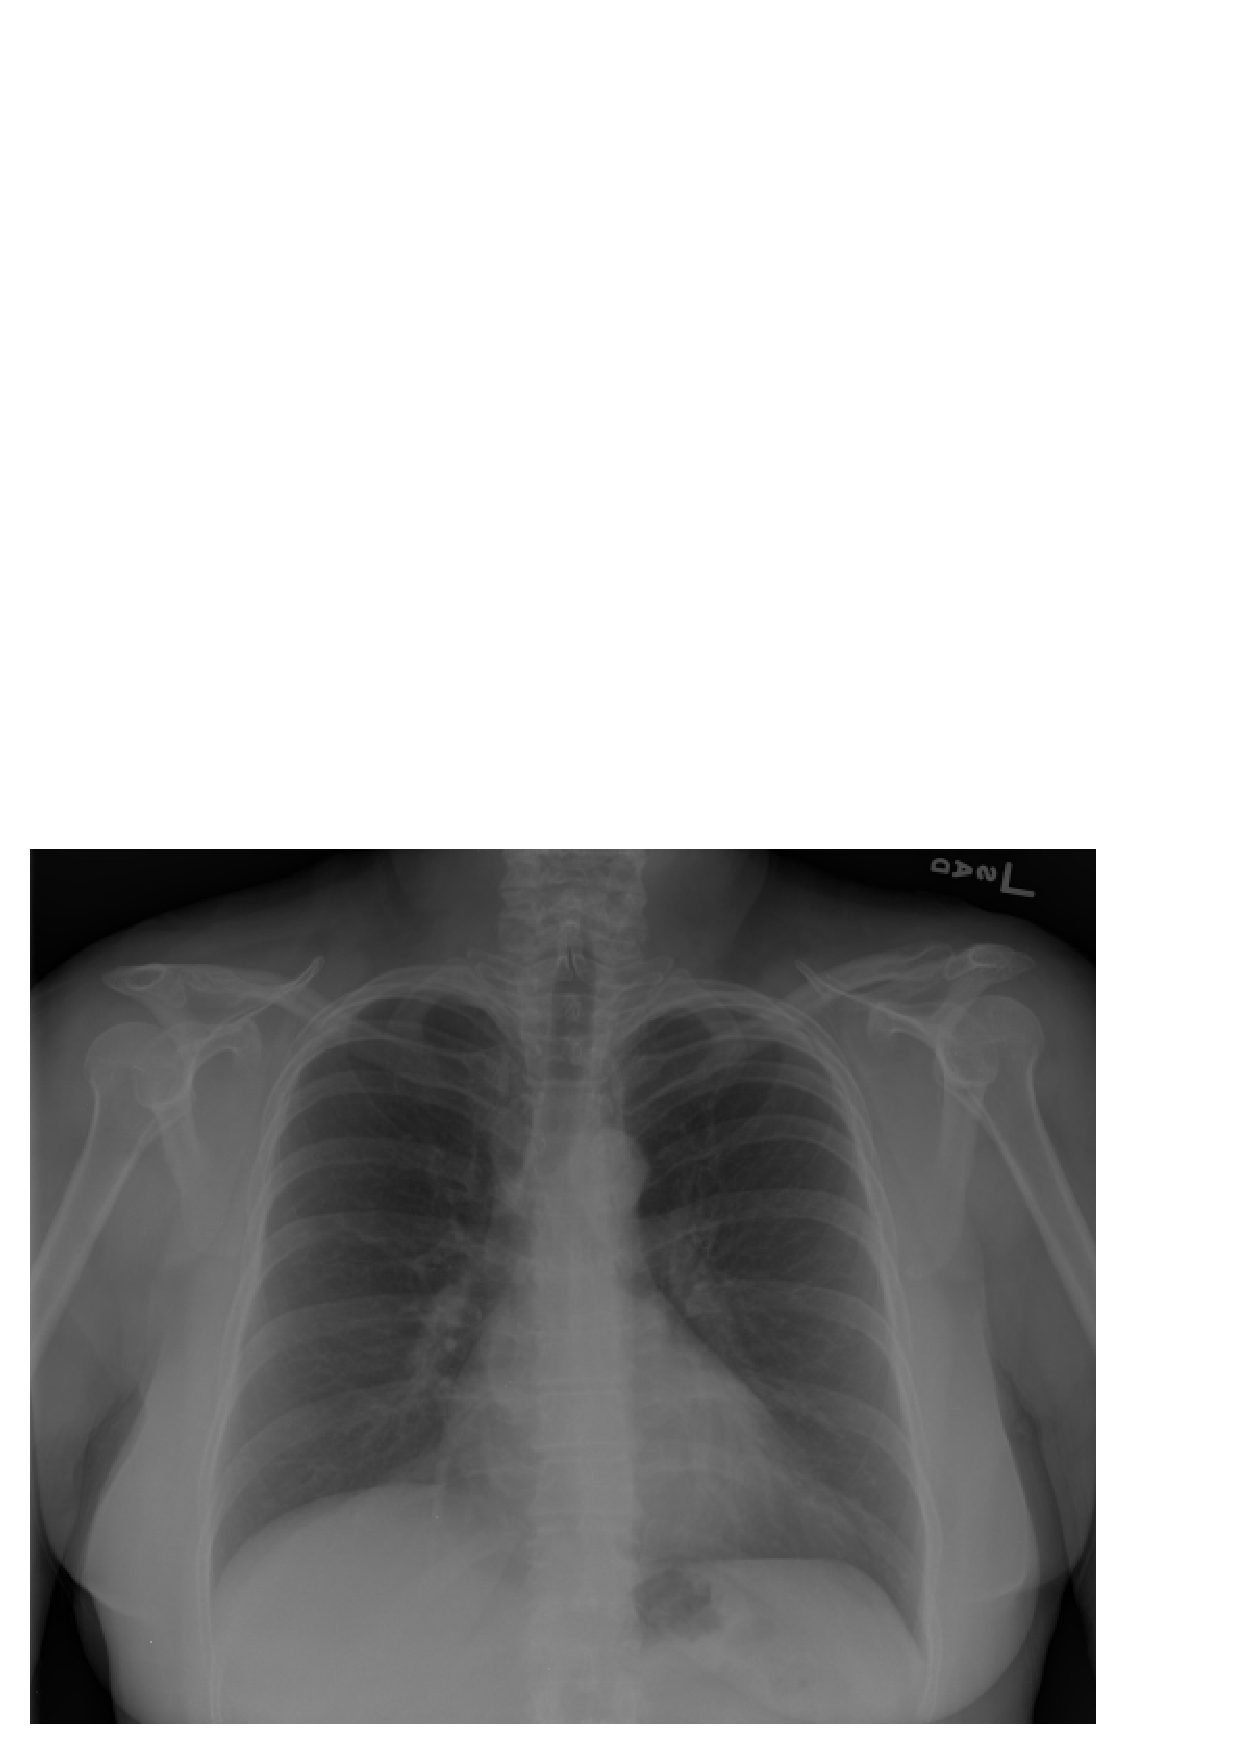
\includegraphics[width=4cm]{Figures/100_IM-0002-1001.png}
   		\captionof{subfigure}{Imagen original}
  	\end{minipage}
  \hspace{1pt}
   \begin{minipage}[t]{0.3\linewidth}  
   		\centering
        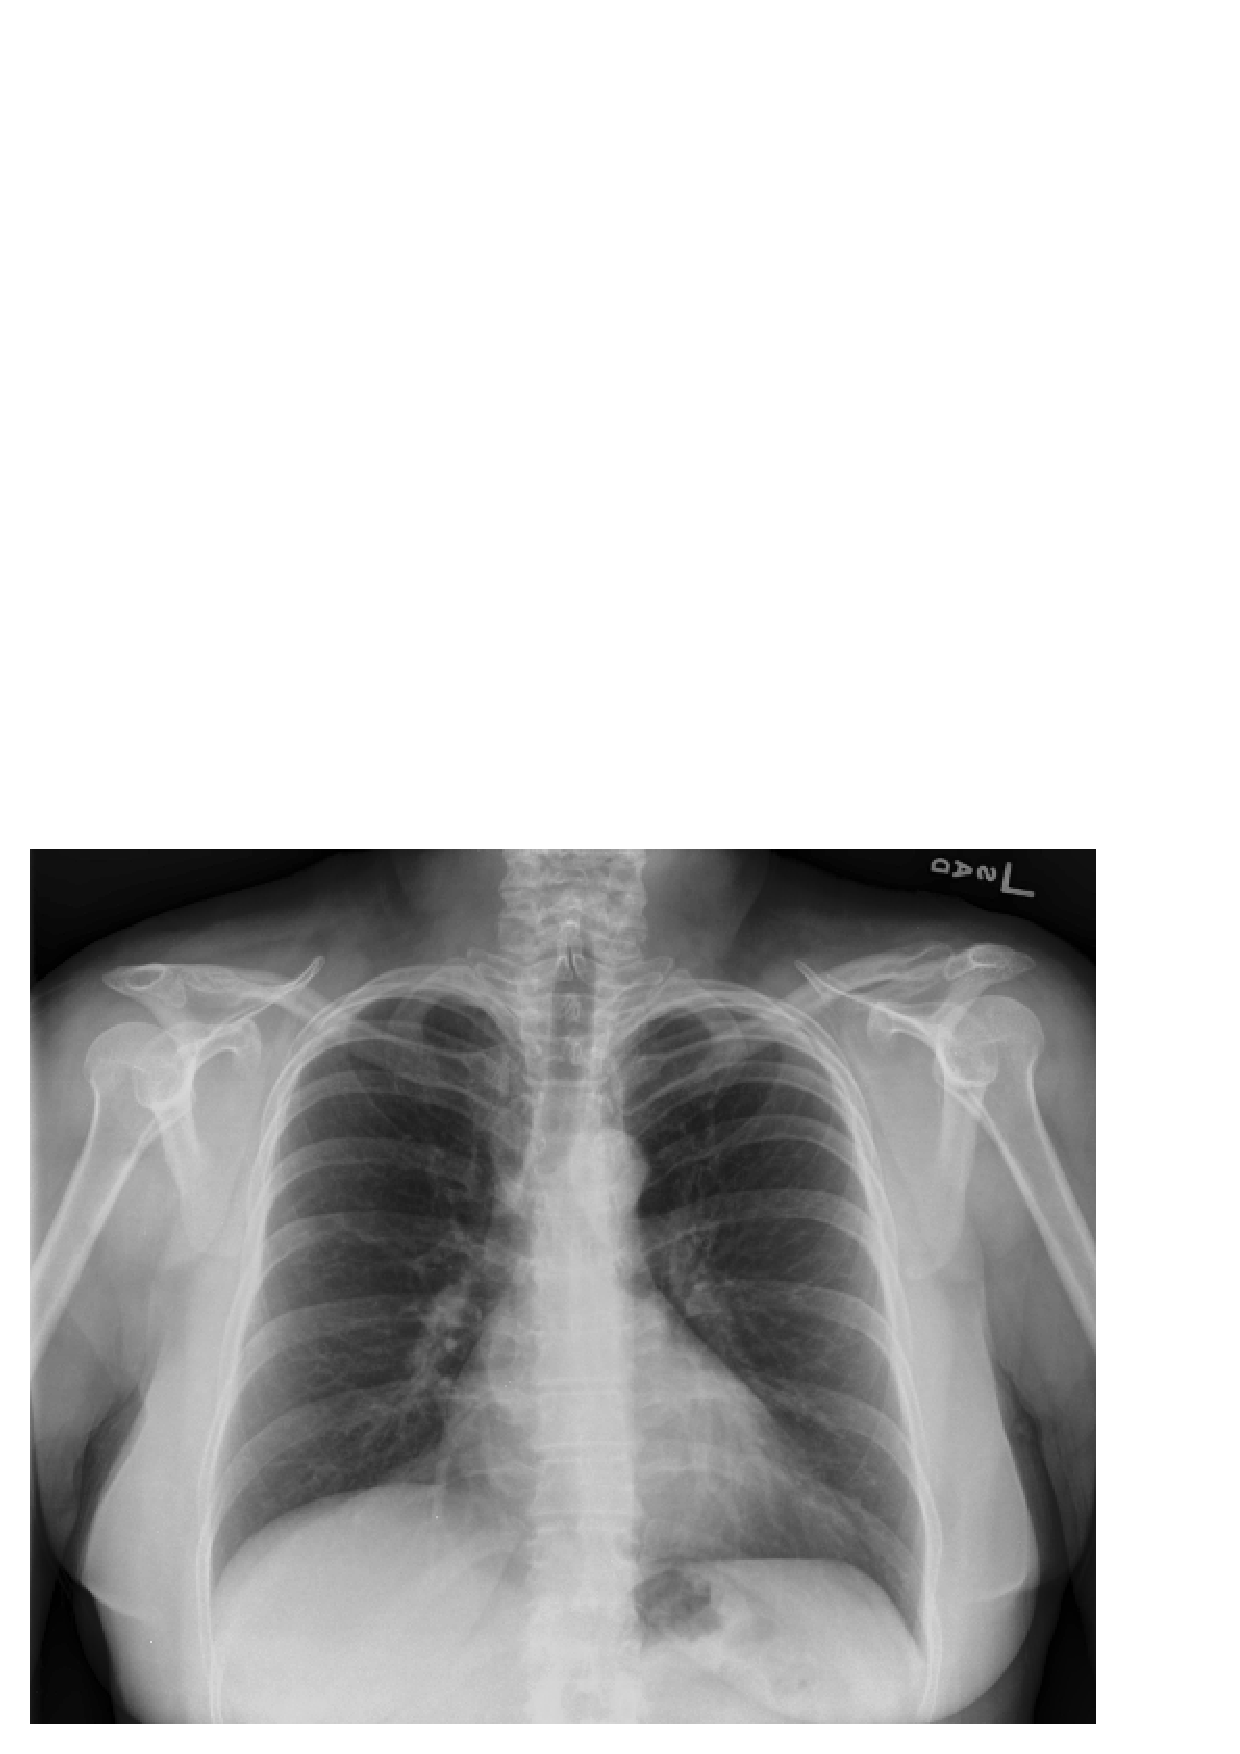
\includegraphics[width=4cm]{Figures/1182-100_IM-0002-1001.png}
   		\captionof{subfigure}{Imagen resultante. $SSIM=0.9688$ $\mathscr{H}=0.7922$}
  	\end{minipage}
  \hspace{1pt}
   \begin{minipage}[t]{0.3\linewidth}  
   		\centering
        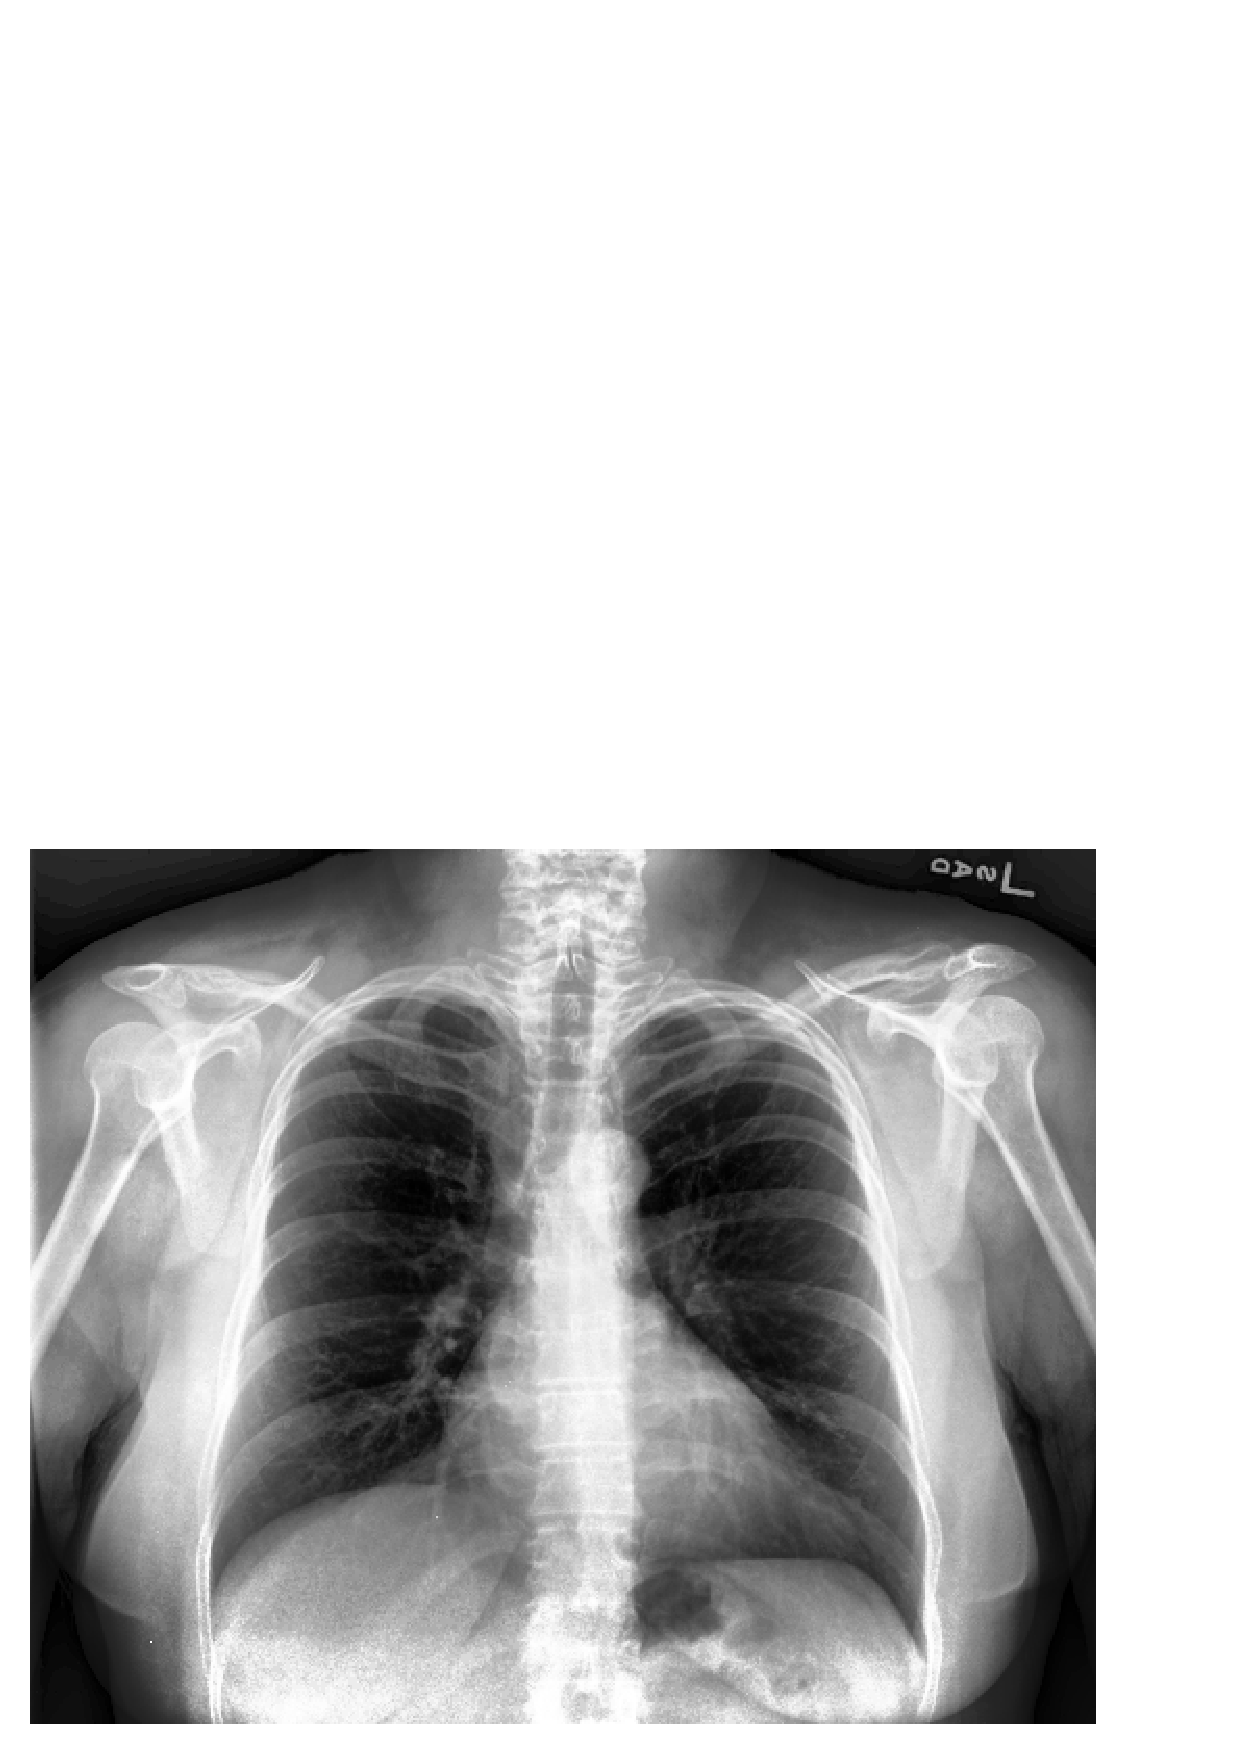
\includegraphics[width=4cm]{Figures/738-100_IM-0002-1001.png}
   		\captionof{subfigure}{Imagen resultante. $SSIM=0.6530$ $\mathscr{H}=0.9933$}
  	\end{minipage}
  \vspace{0.5cm}
    \label{fig:resultado1}
  \captionof{figure}{Resultados de PSO-CLAHE multiobjetivo. }

\end{minipage}

\begin{minipage}[b]{1.0\linewidth}
  
   \begin{minipage}[t]{0.3\linewidth}  
   		\centering
        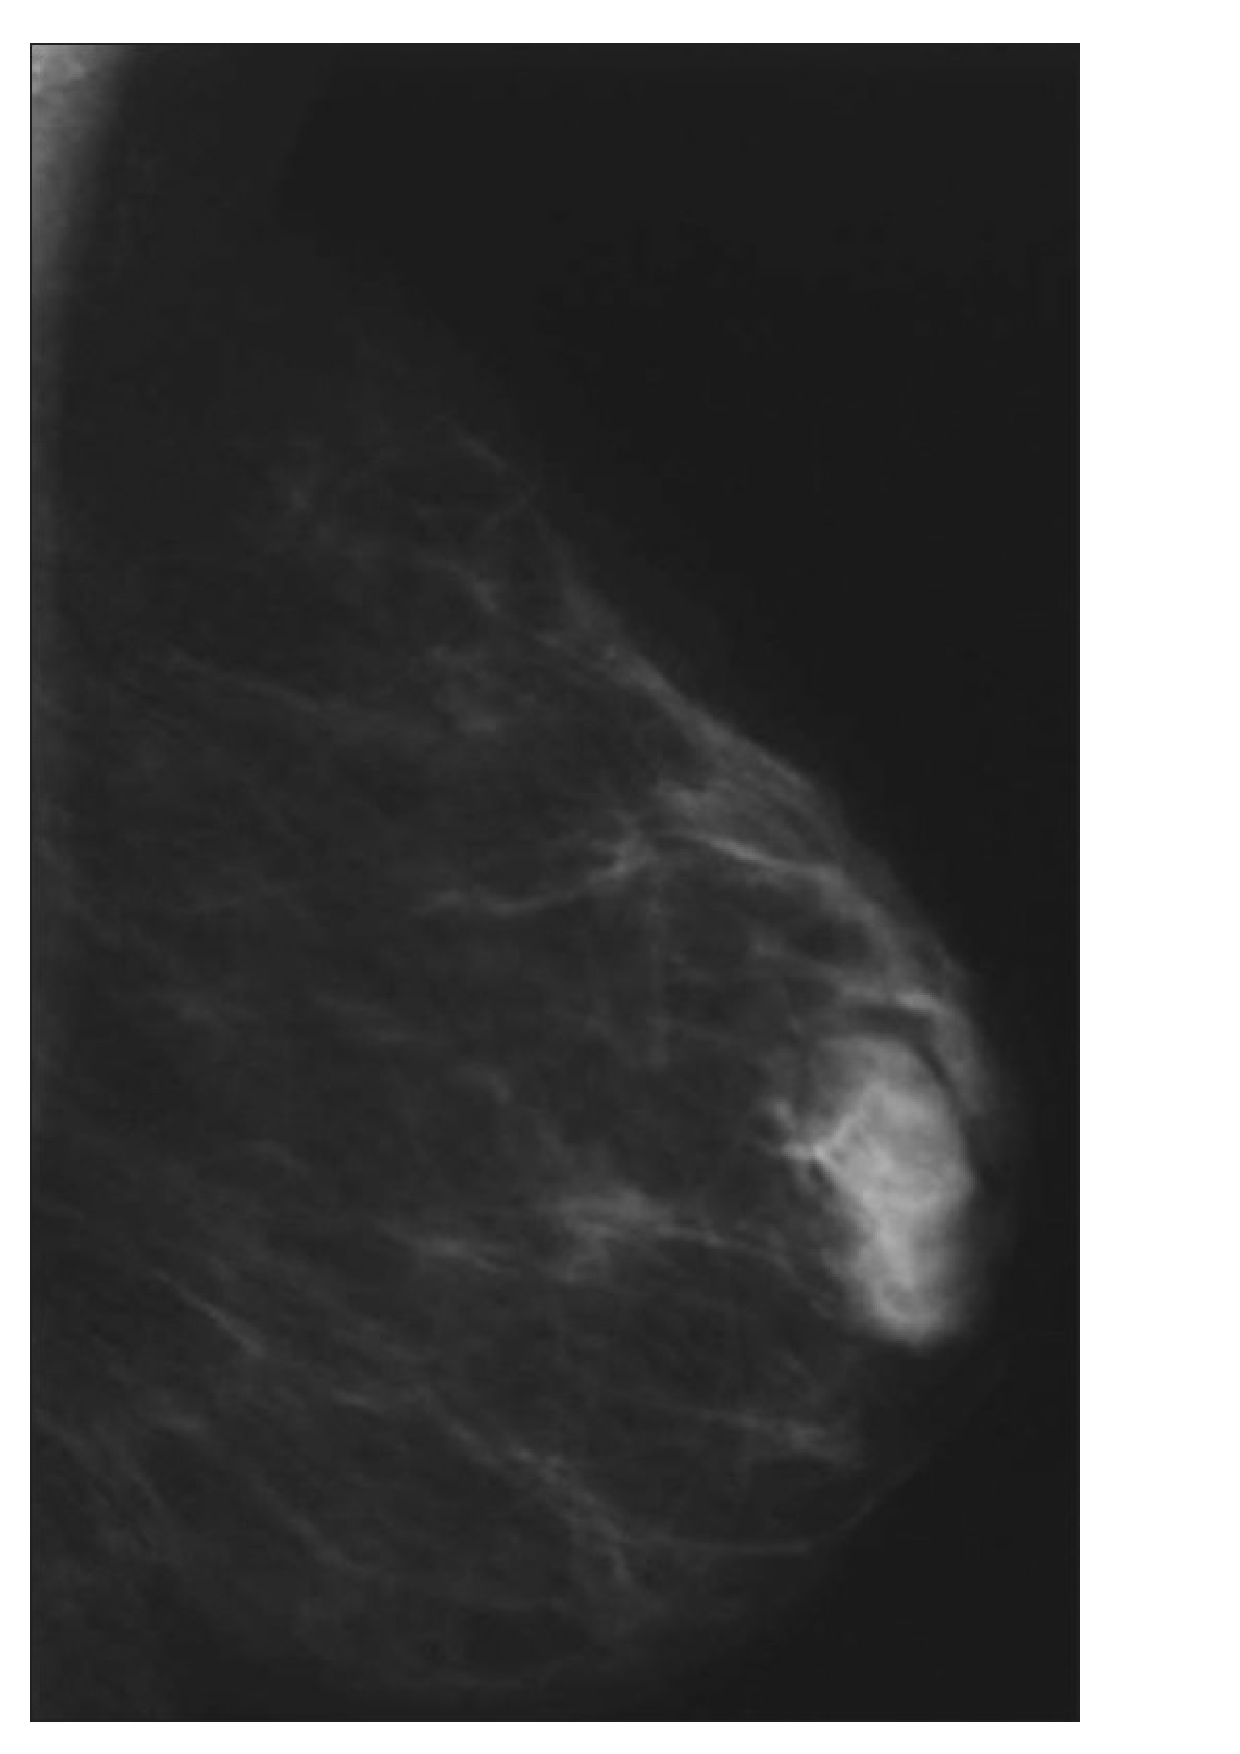
\includegraphics[width=3cm]{Figures/3715982_IJMPO-34-47-g001.png}
   		\captionof{subfigure}{Imagen original}
  	\end{minipage}
  \hspace{1pt}
   \begin{minipage}[t]{0.3\linewidth}  
   		\centering
        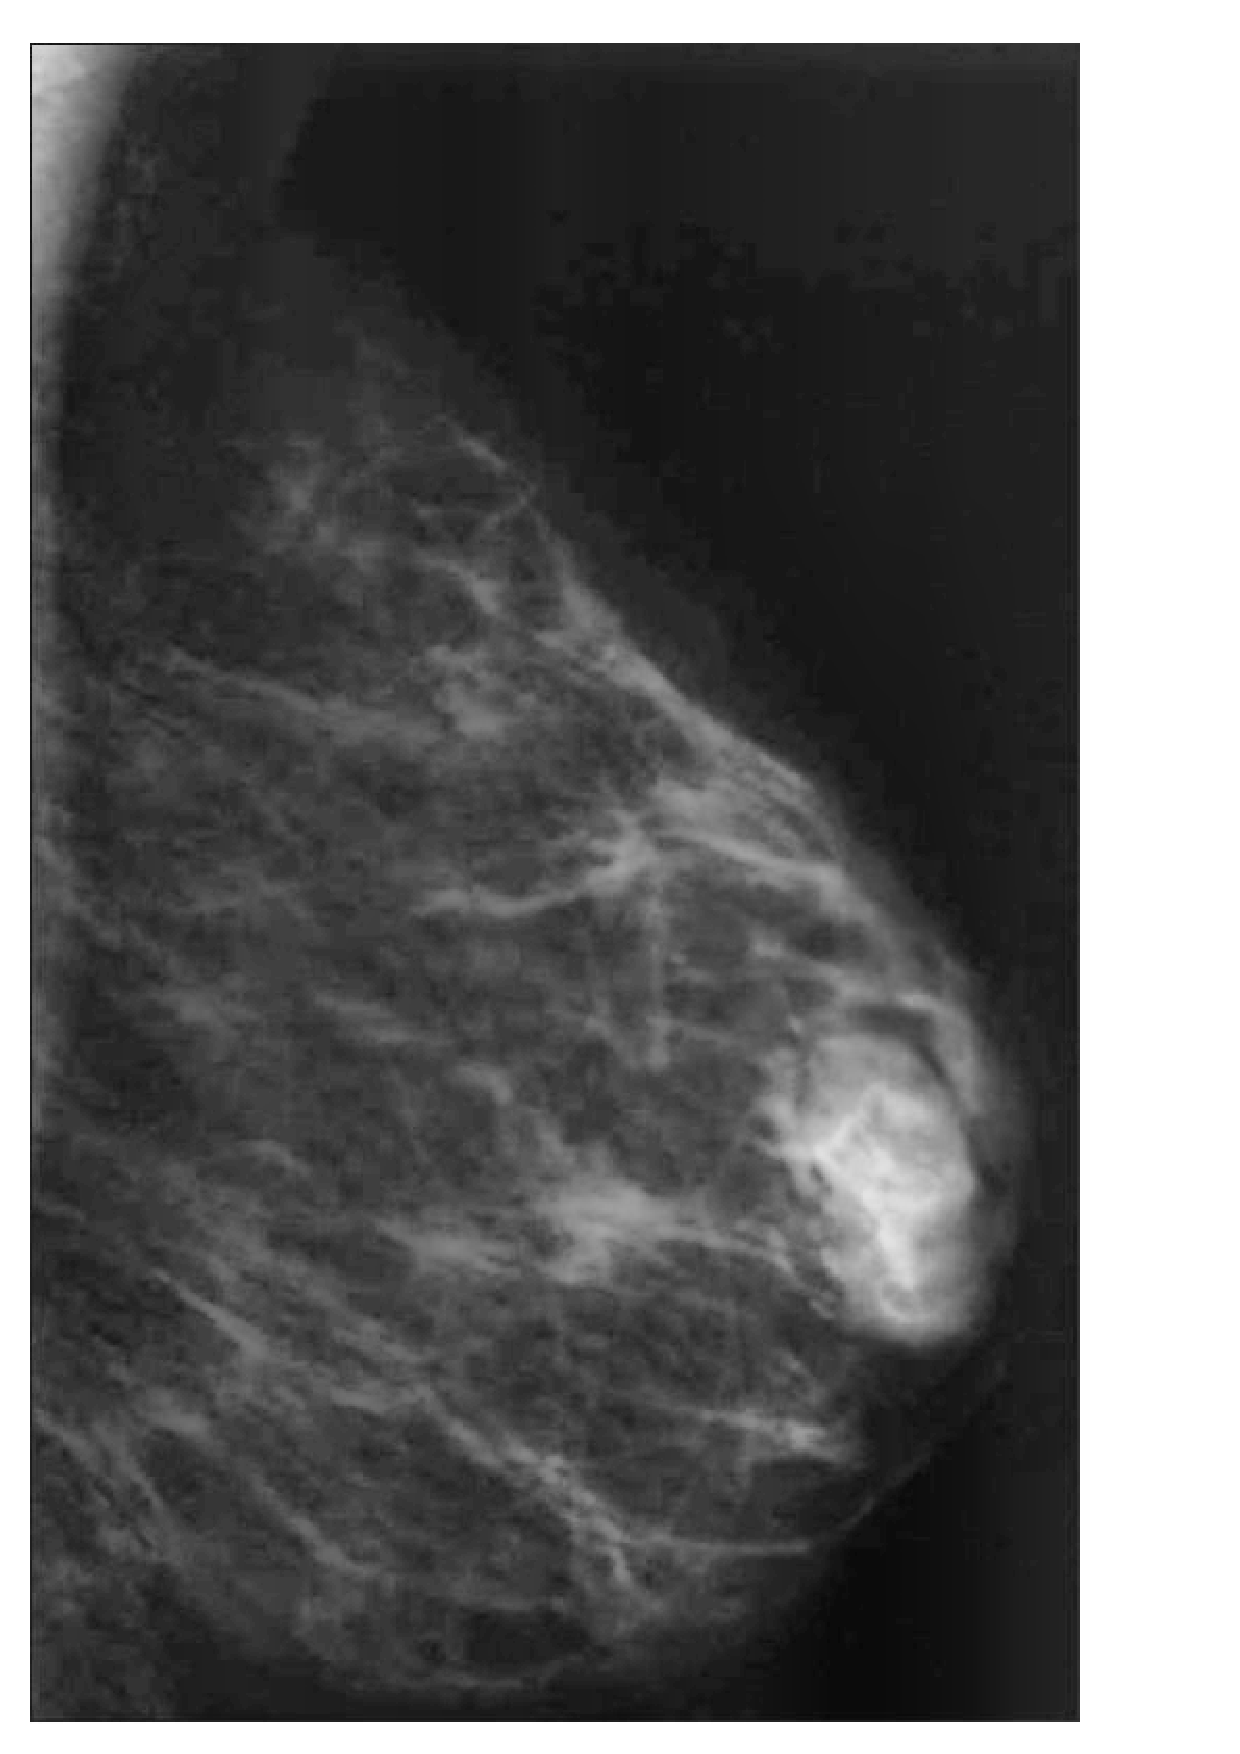
\includegraphics[width=3cm]{Figures/11608-3715982_IJMPO-34-47-g001.png}
   		\captionof{subfigure}{Imagen resultante. $SSIM=0.8032$ $\mathscr{H}=0.8549$}
  	\end{minipage}
   \begin{minipage}[t]{0.3\linewidth}  
   		\centering
        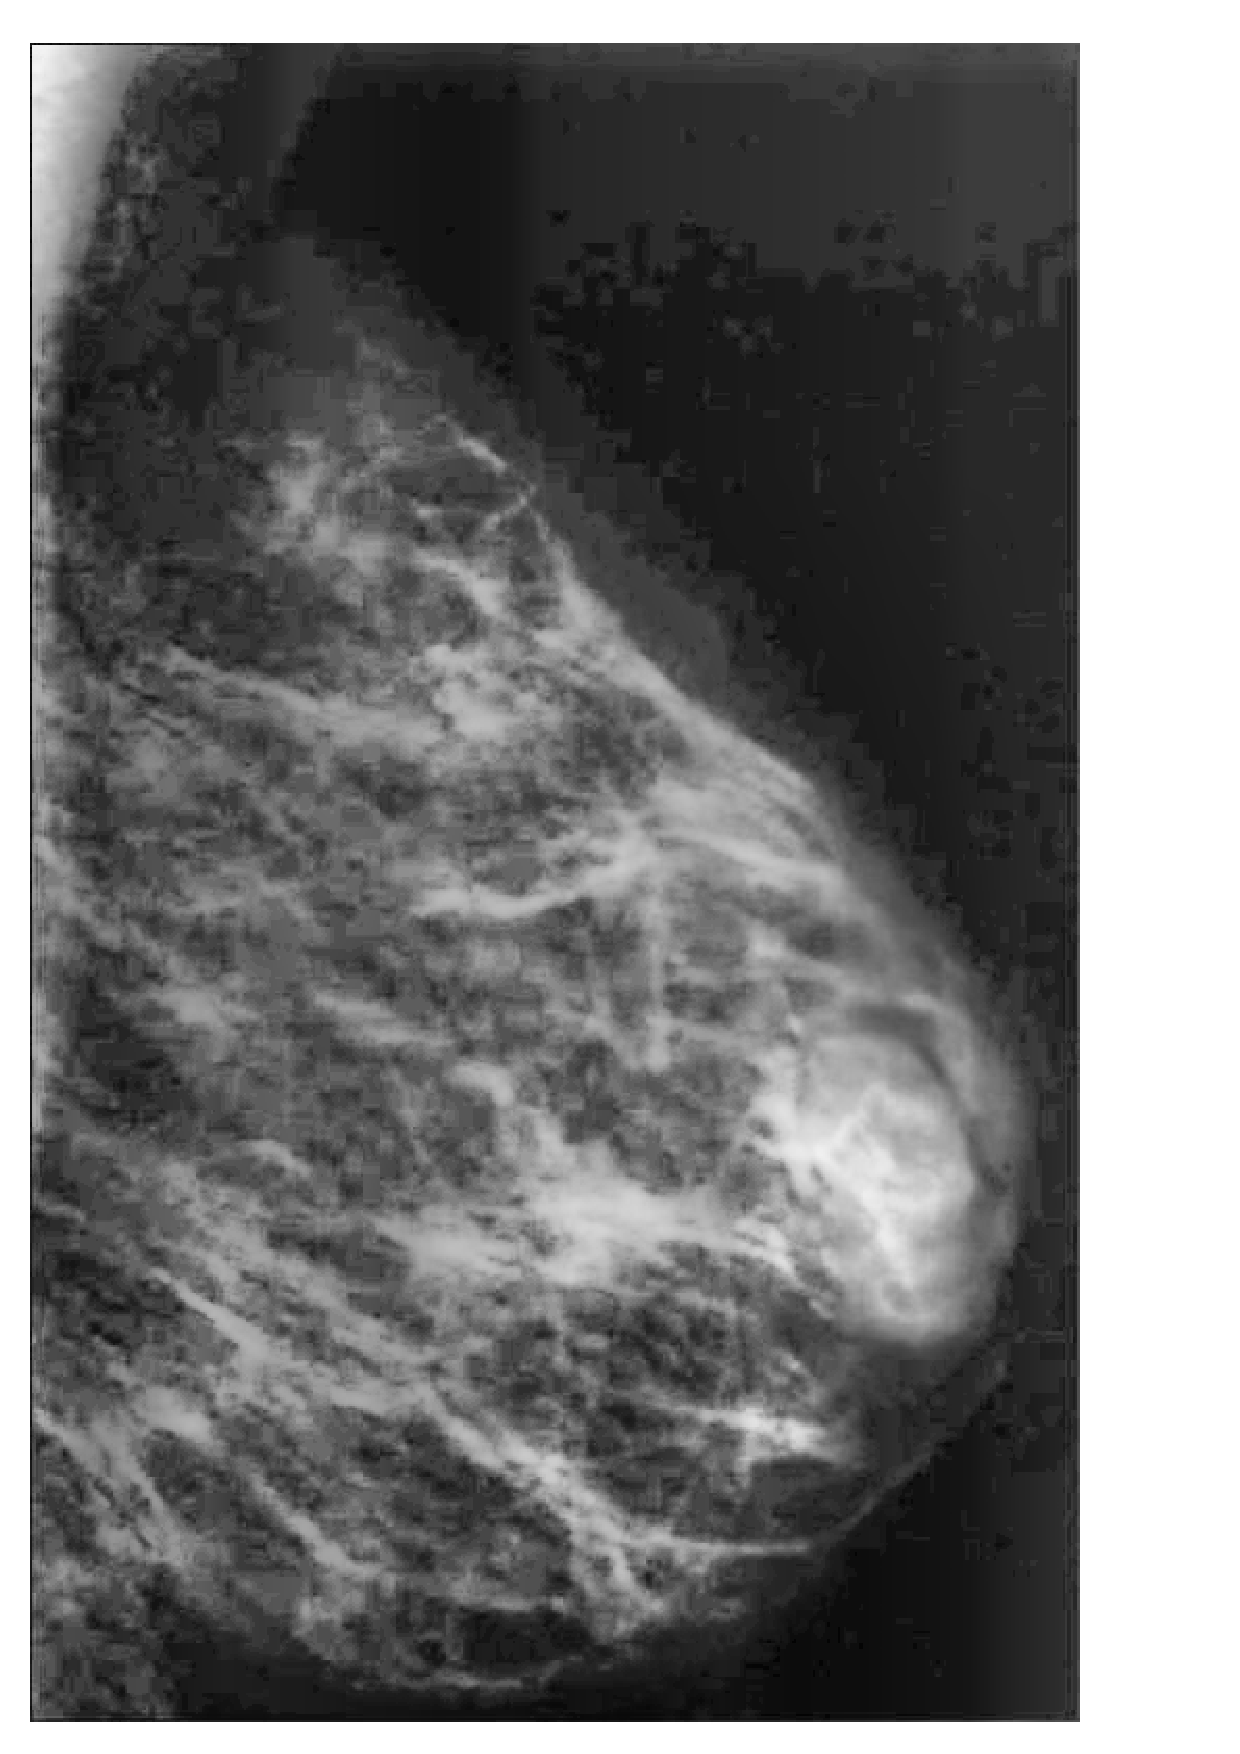
\includegraphics[width=3cm]{Figures/11806-3715982_IJMPO-34-47-g001.png}
   		\captionof{subfigure}{Imagen resultante. $SSIM=0.6059$ $\mathscr{H}=0.9163$}
  	\end{minipage}
  \vspace{0.5cm}
    \label{fig:resultado2}
  \captionof{figure}{Resultados de PSO-CLAHE multiobjetivo. }

\end{minipage}

\begin{minipage}[b]{1.0\linewidth}

   \begin{minipage}[b]{0.48\linewidth}  
   		
        \includegraphics[height=6cm , width=8.5cm]{Figures/pareto-chest.jpg}
   		\captionof{subfigure}{Frente Pareto de la \textbf{Fig. 2}}
  	\end{minipage}
   \hspace{1pt}
   \begin{minipage}[b]{0.48\linewidth}  
   		\centering
        \includegraphics[height=6cm, width=10cm]{Figures/pareto-mamografia.jpg}
   		\captionof{subfigure}{Frente Pareto de la \textbf{Fig. 3}}
  	\end{minipage}
  \vspace{0.5cm}
    \label{fig:resultado3}
  \captionof{figure}{Frentes Pareto para la \textbf {Fig. 2a} y la \textbf {Fig. 3a}. }

\end{minipage}


\twocolumn
\bibliographystyle{IEEEbib}
\bibliography{refs}



\end{document}
